\section{Photometric Redshifts (Photo-$z$s)}
\label{sec:theo_photoz}

A photometric redshift (photo-$z$) is an estimate for the redshift of an astronomical object, such as a galaxy or quasar, using its photometry $m_i$ in various standard filters $i$. This is in contrast to the spectroscopic redshift (spec-$z$) where the shift in a spectral feature, such as an emission or absorption line, along the spectrum is determined, allowing the determination of $z$ directly from its definition in (\ref{redshift}). 

The technique is an old idea that originated in the 1960s (\citet{Baum1962, Puschell1982, Koo1985, Loh1986, Connolly1995}), but was later largely replaced by spec-$z$s. However, it has made a come-back in the last two decades, as a result of new large sky surveys (section \ref{sec:surveys}), since it provides galaxy redshifts substantially faster than the spectroscopic technique, especially when the observed objects are faint. Moreover, photo-$z$ based surveys do not suffer the incompleteness of the target selection needed in spectroscopic surveys, since all objects in the telescope's field-of-view are registered at once (in contrast to spectroscopic surveys where the spectrograph must be pointed to each target individually and some objects may be ignored). The disadvantage is that the precision for these sorts of measurements is typically $\sigma_z \sim 0.05-0.10$, and are less reliable than spectroscopic determinations.  

There are basically two types of methods to determine photometric redshifts: the template-fitting methods (e.g. Hyperz, \citet{Bolzonella2000}; BPZ, \citet{Benitez2000} \& \citet{Coe2006}; LePhare, \citet{Ilbert2006}; EAZY, \citet{Brammer2008}; LRT, \citet{Assef2008}; GALEV and GAZELLE, \citet{Kotulla2008}), and the training-set methods (e.g. ANNz, \citet{Collister2004}; ArborZ, \citet{Gerdes2010}; TPZ, \citet{CarrascoKind2013};  Li, \citet{Li2008}; Carliles, \citet{Carliles2010}). In some cases a method can belong to the two previous groups at the same time (e.g. Kernelz; \citet{Wolf2014}), so they are called hybrid methods. In this thesis we will focus on the template-fitting methods leaving the training-set and hybrid methods as alternatives. 

In order to calibrate the goodness of the photo-$z$ determinations one typically uses a spectroscopic sample with known spec-$z$ redshifts, taken as fiducial. In Fig.~\ref{fig:phat_photoz} we show several scatter plots of $\Delta z \equiv z_{ph} - z_{sp}$ vs. $z_{sp}$, where $z_{ph}$ is the photometric redshift and $z_{sp}$ the spectroscopic one, for different photo-$z$ methods applied on the same galaxy sample. If the photo-$z$ determination was perfect, all the points would be at $\Delta z = 0$ (over the black line). However, they are actually spread out around this value. The problem is that they are not typically spread out according to a Gaussian profile, but rather to a more complex distribution with asymmetries, bias, double maxima, etc., which needs to be characterized carefully. Moreover, these $\Delta z$ distributions can rapidly change their shape with redshift, spectral type, magnitude, etc. Usually, these complex distributions are characterized using three different metrics: the bias (mean, median, etc.), which tell us how the overall shape of the distribution is offset from $\Delta z =0$, the precision (RMS, $\sigma_{68}$, etc.), which tells us how dispersed are the photo-$z$ determinations from these offsets, and the outlier fraction, which tells us the rate of determinations much worse than expected (that is, the extend of the tails of the $\Delta z$ distribution).
\begin{figure}
\centering
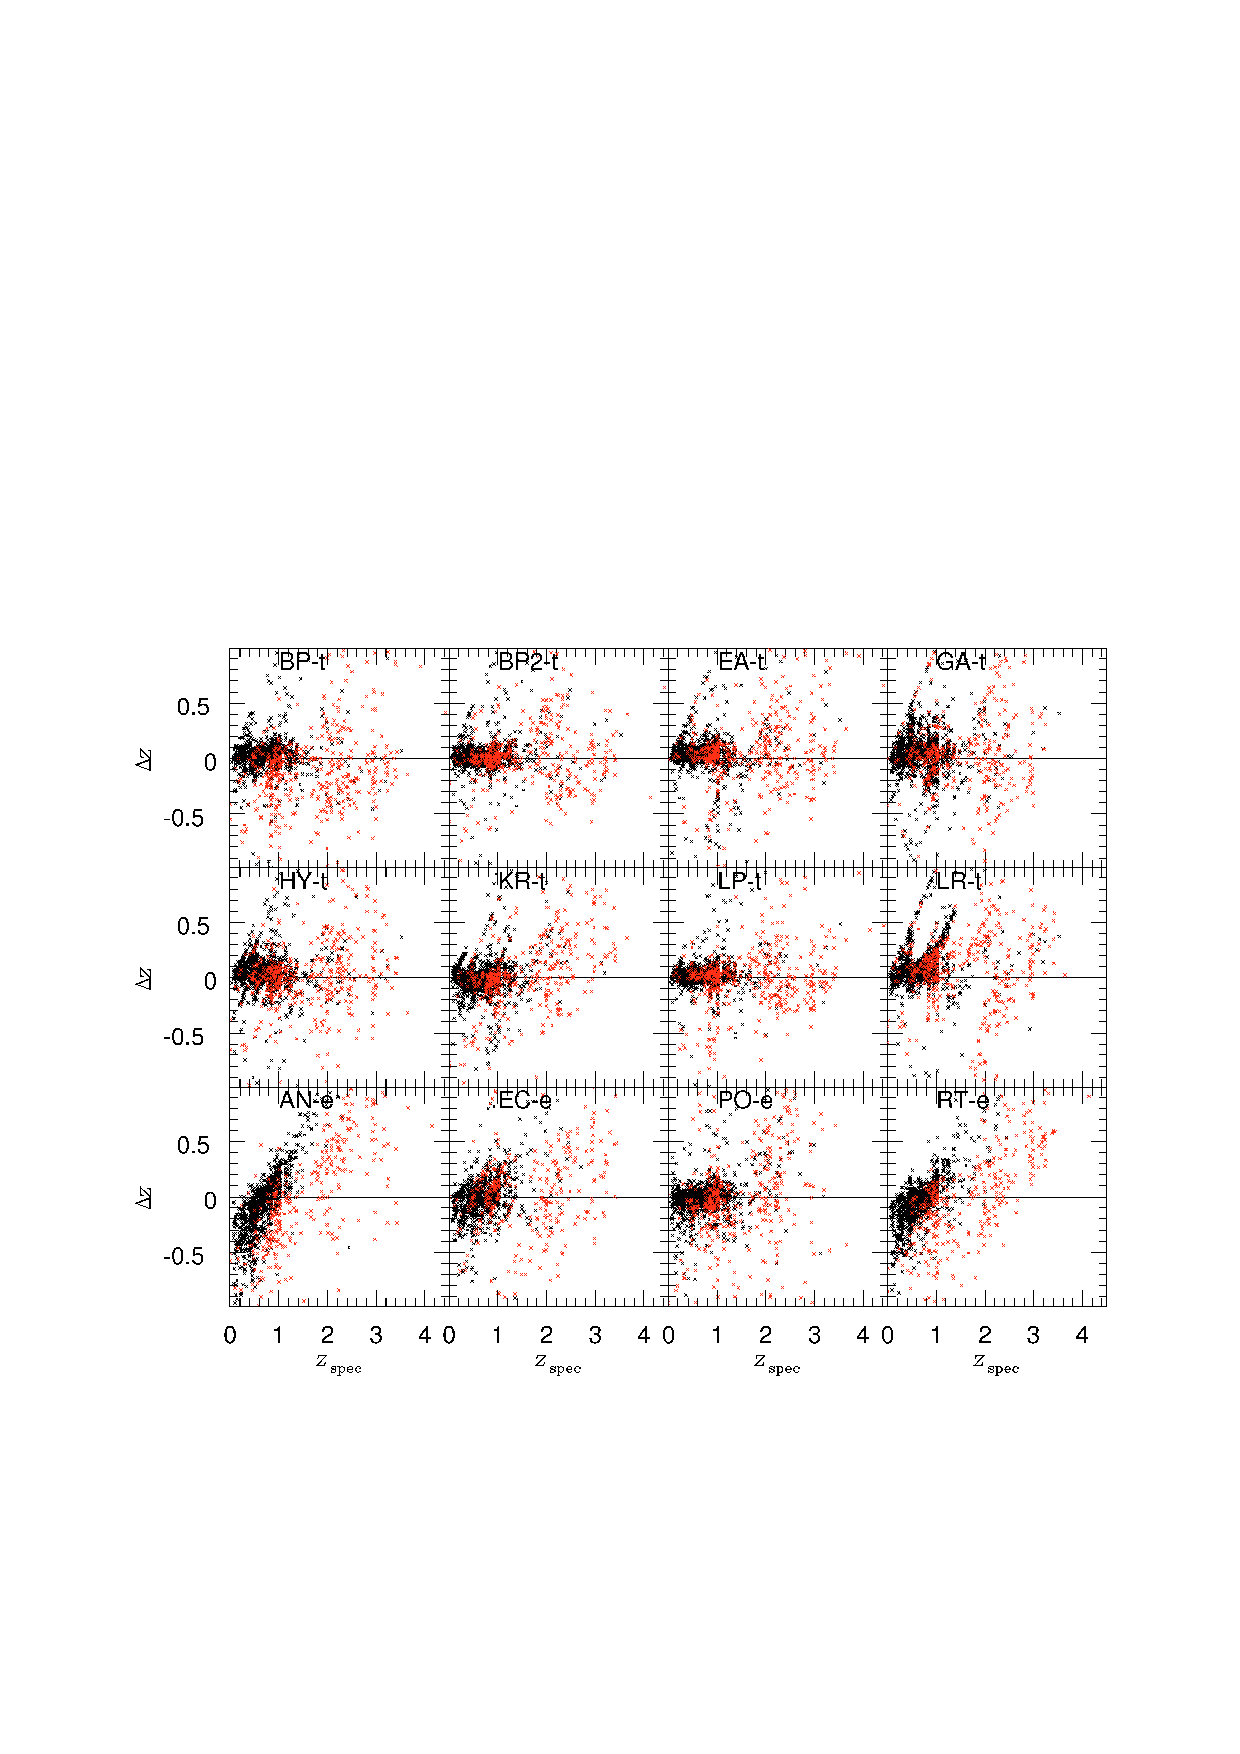
\includegraphics[width=140mm]{./plots/phat_dzvsz.pdf}
\caption{Scatter plots $\Delta z \equiv z_{ph} - z_{sp}$ vs. $z_{sp}$, where $z_{ph}$ is the photometric redshift and $z_{sp}$ is the spectroscopic redshift, of galaxies from the Great Observatories Origins Deep Survey northern field (GOODS-N, \citet{Giavalisco2004}) in the PHAT1 test \citep{Hildebrandt2010} for different photo-$z$ methods: BPZ (BP-t or BP2-t, \citet{Benitez2000}), EASY (EA-t, \citet{Brammer2008}), GALEV and GAZELLE(GA-t, \citet{Kotulla2008}), Hyperz (HY-t, \citet{Bolzonella2000}), Kernelz (KR-t), Le Phare (LP-t, \citet{Arnouts1999} \& \citet{Ilbert2006}), LRT (LR-t, \citet{Assef2008}), ANNz (AN-e, \citet{Collister2004}), Wolf (EC-e, \citet{Wolf2014}), Li (PO-e, \citet{Li2008}) and Carliles (RT-e, \citet{Carliles2010}). Faint objects with $R\ge24$ are shown in red. Figure from \citet{Hildebrandt2010}.}
\label{fig:phat_photoz}
\end{figure}

\subsection{Template-Fitting Methods}
The template-fitting methods compare the observed fluxes $F_i$ of the celestial object in different passbands $i$ with the predicted fluxes $F_i^t(z)$ obtained by redshifting a set of spectral templates, $f^t(\lambda) \rightarrow f^t(\lambda/1+z)$, and integrating them in the passbands $R_i(\lambda)$ through Eq.~(\ref{eq:flux}). The photometric redshift value will be the redshift $z_{ph}$ that, for example, minimizes the following $\chi^2$:
\begin{equation}
\chi^2(z,t; F_i)=\sum_i {(F_i -  F_i^t(z))^2 \over  \sigma_F^2},
\end{equation}
where $\sigma_{F_i}$ is the error of the measured flux $F_i$. Figure~\ref{fig:sdss_filt} provides a visual explanation of what this $\chi^2$ minimization means. According to the shape of the Vega spectrum, which abruptly starts growing from $\sim$4000~\AA, it is easy to see that the less flux will pass through bluer filters, the more shifted to redder wavelenghts the spectrum will be. Therefore, if we know beforehand the shape of the spectrum of the object we are observing, we only have to find how redshifted it would have to be in order to recover the observed fluxes. That is why prominent spectral features with an abrupt change on the spectral density flux, such the 4000\AA \ break in elliptical galaxies (see Fig.~\ref{pau_templates}), are especially good for photo-$z$ determination (this is also valid for training-set methods).
 
The goodness of the photo-$z$ determination will depend on how well the spectral templates represent the observed galaxy population. If the sample of galaxies to be studied has a wide spectral-type diversity, it is desirable to use a set of templates that covers all possible spectral types. If, on the contrary, the sample only contains galaxies of a single spectral type, it is desirable to use only templates corresponding to the same spectal type in order to avoid spectral type confusions. Commonly used template sets are the \citet{Coleman1980} Spectral Energy Densities (SEDs) which are derived observationally, or those of \citet{Bruzual1993}, derived from population synthesis models. Some examples of galaxy templates can be found in Fig.~\ref{pau_templates}, which contains spectral types ranging from early-types to late-type galaxies, and Fig.~\ref{2slaq_templates}, which is more focused on early-type galaxies. Note that galaxy templates evolve smoothly through different spectral types starting from elliptical galaxies, then to spirals, irregulars and finally reaching starburst galaxies. For this reason, the accuracy with which we want to resolve different spectral types can be tuned by adding more or less interpolated templates between the original ones.


\subsection{Training-Set Methods}
The training-set methods derive a parametrization $z=f(m_i;p_j)$ for the redshift, where $p_j$ are some parameters, as a function of the photometry $m_i$ in the different bands $i$. The values of the parameters $p_j$ are deduced by fitting $z=f(m_i;p_j)$ to a training set of galaxies, for which we have both photometry and spectroscopic redshifts, representative of the target set. The training set could be obtained empirically or derived from a set of spectral templates (as in the template-fitting methods) or from simulated catalogs (e.g. \citet{Vanzella2004}). The training method will only be reliable when it is applied to galaxies within the ranges of redshift and spectral type of the training set. 

The parametrization $z=f(m_i;p_j)$ can be expressed throughout a polynomial (e.g. \citet{Connolly1995}; \citet{Sowards-Emmerd2000}), an artificial neural network \citep{Collister2004}, boosted decision trees \citep{Gerdes2010}, random forests \citep{Carliles2010}, etc. Additionally, it can be generalized to any other properties of the galaxies besides the redshift, such us the spectral type, the ellipticity or even the probability to be either a galaxy or a star.

\subsection{Bayesian photometric redshifts}
The presence of some similar prominent spectral features at significantly different wavelengths can lead to degeneracies in color space and, consequently to confusions in the photo-$z$ determination. When this happens, photo-$z$s can result much higher or lower than actual redshifts, which are known as catastrophic redshift determinations.  

As in the training-set methods, a representative subset of the photometric target sample for which we know their spectroscopic redshifts could tell us beforehand how galaxies are actually distributed in redshift, and mitigate the catastrophic redshift determinations. According to \citet{Benitez2000} this can be done in template-fitting methods by using Bayesian statistics as follows:
\begin{equation}
p(z|m_j) = \sum_t p(z,t|m_j) \propto \sum_t L(m_j|z,t) \, \Pi(z,t)  \, ,
\label{pz_intro}
\end{equation}
where $p(z|m_j)$ is the posterior probability density distribution (pdf) that the galaxy has redshift $z$ when its photometry is $\lbrace m_j \rbrace$, $L(m_j|z,t) \propto \exp \lbrace -1/2 \chi^2(z,t; F_j) \rbrace$ is the likelihood that the galaxy has photometry $\lbrace m_j \rbrace$ when the redshift is $z$ and the spectral type is $t$, and $\Pi(z,t)$ is the prior probability that the galaxy has redshift $z$ and spectral type $t$. The prior probability $\Pi(z,t)$ must be an empirical function that describes the redshift and spectral type distributions of the spectroscopic training set. 

In Fig.~\ref{fig:prior_parts} and in descending order, we show the likelihood $L(m_j|z,t)$, the prior probability $\Pi(z,t)$, the product of both $p(z,t|m_j)$ and the posterior probability $p(z|m_j)$ of the photo-$z$ determination of an irregular galaxy at $z=0.28$ and magnitude $I\sim26$ using BPZ \citep{Benitez2000}. According to the likelihood alone the galaxy should be a spiral galaxy at redshift $z_{ph}\sim2.7$. However, the prior probability function suppresses the high redshift peak, moving the posterior pdf to a more reasonable redshift with the right spectral type.
\begin{figure}
\centering
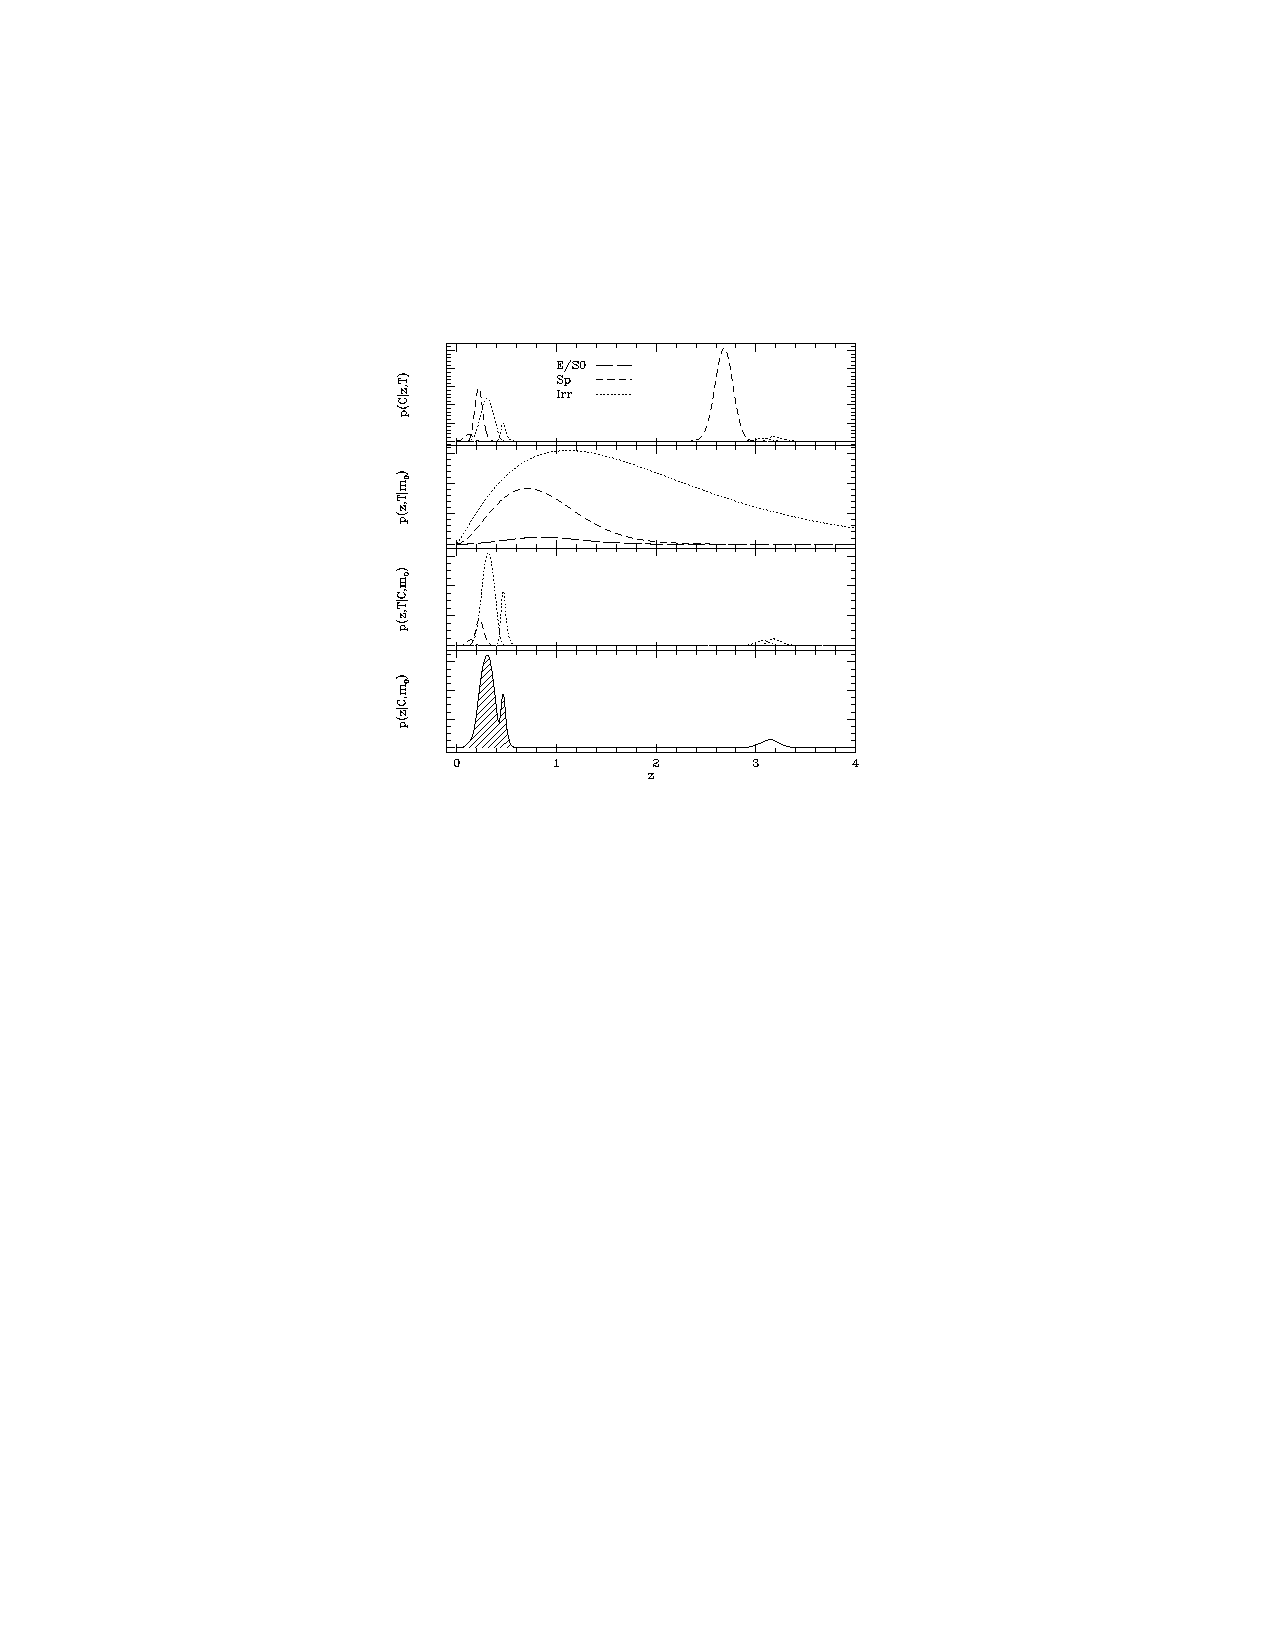
\includegraphics[width=100mm]{./plots/prior.pdf}
\caption{In descending order: the likelihood $L(m_j|z,t)$, the prior probability $\Pi(z,t)$, the product of both $p(z,t|m_j)$ and the posterior probability $p(z|m_j)$ of the photo-$z$ determination of a galaxy at $z=0.28$ using the BPZ code. The prior probability helps suppress the high redshift peak at $z\sim2.7$ in the likelihood and moves the galaxy closer to its actual redshift. Figure from \citet{Benitez2000}.}
\label{fig:prior_parts}
\end{figure}

In the scatter plot $z_{ph}$ vs. $z_{zp}$ on the left of Fig.~\ref{fig:prior}, we can see examples of catastrophic redshift determinations: four dots at $z_{sp}\sim 0.5$ whose photo-$z$ is around 3, as well as a dot at $z_{sp}\sim3$ when $z_{ph}$ is close to 0.5. Once the prior probability is used (scatter plot on the right), all these points get closer to the diagonal.
\begin{figure}
\centering
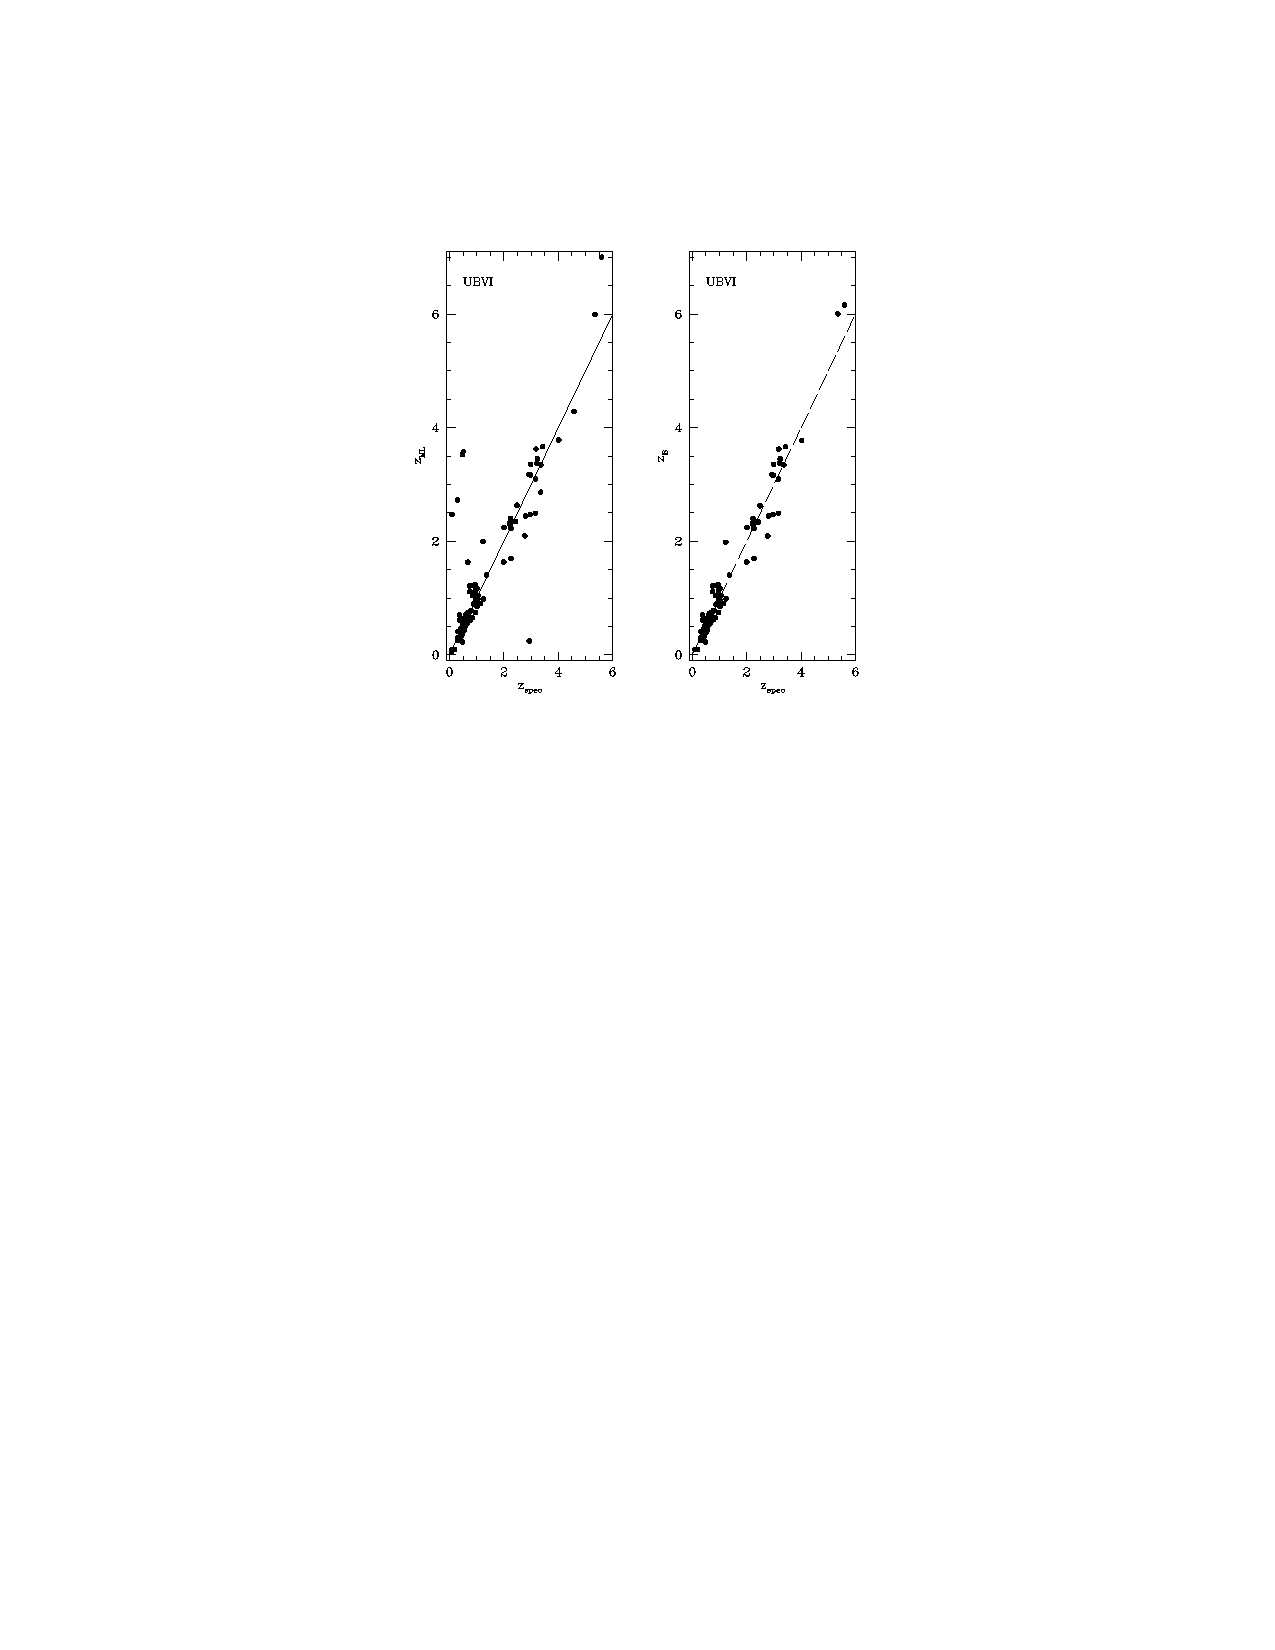
\includegraphics[width=90mm]{./plots/prior_catastrophic.pdf}
\caption{The $z_{ph}$ vs. $z_{sp}$ scatter plots for the photo-$z$s obtained with the BPZ code when run on 101 galaxies in the Hubble Deep Field (HDF, \citet{Williams1996}) spectroscopic sample with photometry on the Hubble Space Telescope (HST) bands $UBVI$. The left plot corresponds to photo-$z$s obtained by maximizing only the likelihood in (\ref{pz_intro}), while in the right plot the whole posterior probability is maximized. Clearly, Bayesian statistics help reduce the presence of catastrophic redshift determinations (the points far away from the diagonal). Figure from \citet{Benitez2000}.}
\label{fig:prior}
\end{figure}

Besides reducing the catastrophic redshift determination rate, the Bayesian approach returns a probability density function $p(z|m_j)$ which contains much more information than a single photo-$z$ value. In subsection~\ref{sec:lss} we saw that spatial galaxy-galaxy correlations at different redshifts are useful to trace the evolution of the large scale structure in the Universe over time and, finally, determine cosmological parameters. These different redshifts are selected through photo-$z$ bins $i$ of width comparable to the photo-$z$ precision whose galaxies' true redshift distribution is $N_i(z)$. These distributions must be known in order to compute predictions of, for example, the angular correlations $\omega_{G_i G_j}(\theta)$ through Eq.~\ref{eq:corr_prediction}. The easiest way to obtain the shape of these distributions is by splitting galaxies of a representative spectroscopic sample into the same photo-$z$ bins used for the target sample, and then compute the resulting spec-$z$ distribution in each bin. However, sometimes such spectroscopic sample is not available. On those cases, the stacking of all the $p(z|m_j)$ of the galaxies inside the photo-$z$ bin can give a shape very close to the actual $N_i(z)$ \citep{Bonnett2013}.

\subsection{Photo-$z$ quality estimator (\textit{odds})}
Photo-z codes, besides returning a best estimate for the redshift, typically also return an indicator of the photo-$z$ quality. It can be simply an estimation of the error on $z_{ph}$, or something more complex, but the aim is the same. In \texttt{BPZ} this indicator is called \textit{odds}, and it is defined as
\begin{equation}
odds = \int^{z_{ph}+\delta z}_{z_{ph}-\delta z}p(z|m_j)dz \, ,
\label{odds}
\end{equation}
where $\delta z$ determines the redshift interval where the integral is computed. \textit{Odds} can range from 0 to 1, and the closer to 1, the more reliable is the photo-$z$ determination, since $p(z|m_j)$ becomes sharper and most of its area is enclosed within $z_{ph}\pm \delta z$. On the right plot of Fig.~\ref{fig:odds} we illustrate this by showing two examples of $p(z|m_j)$ for two LRGs in the 2SLAQ sample (see subsection~\ref{sec:sdss}), whose spectroscopic redshift is roughly the same, $z_{sp} \sim 0.5$, but the returned photo-$z$ by BPZ is clearly distinct. While for one galaxy (green curve) the measured photo-$z$ is very close to the spectroscopic redshift, for the other (blue curve) it differs by $\sim0.1$, something that we were already warned of by the colored areas under the curves, which show the interval where the odds is computed. Note how in the first case the relative area is clearly larger (97\%) than in the second (51\%). Also note that in the second case the pdf shows a small bump pointing to the right redshift, which tells us, that there may have been a confusion on the template matching similar to that in Fig.~\ref{fig:prior_parts} causing a catastrophic redshift determination, something that could be fixed by using a prior.

Since \textit{odds} are a proxy for the photo-$z$ quality, we should expect a correlation between the \textit{odds} and $|\Delta z|$, in the sense that higher \textit{odds} should correspond to lower $|\Delta z|$. On the left plot of Fig.~\ref{fig:odds} there is a scatter plot of \textit{odds} (shown as $p$) vs. $|\Delta z|$ for galaxies in the Hubble Deep Field (HDF). We see that catastrophic outliers, defined as $|\Delta z|>1$, have rather low \textit{odds} values. Points under the dashed line comprise 25\% of the catalog. Most of the catastrophic outliers are in this region, so they can be removed by setting an appropriate threshold on the \textit{odds} value and removing all those galaxies below it.
\begin{figure}
\centering
\begin{tabular}{cc}
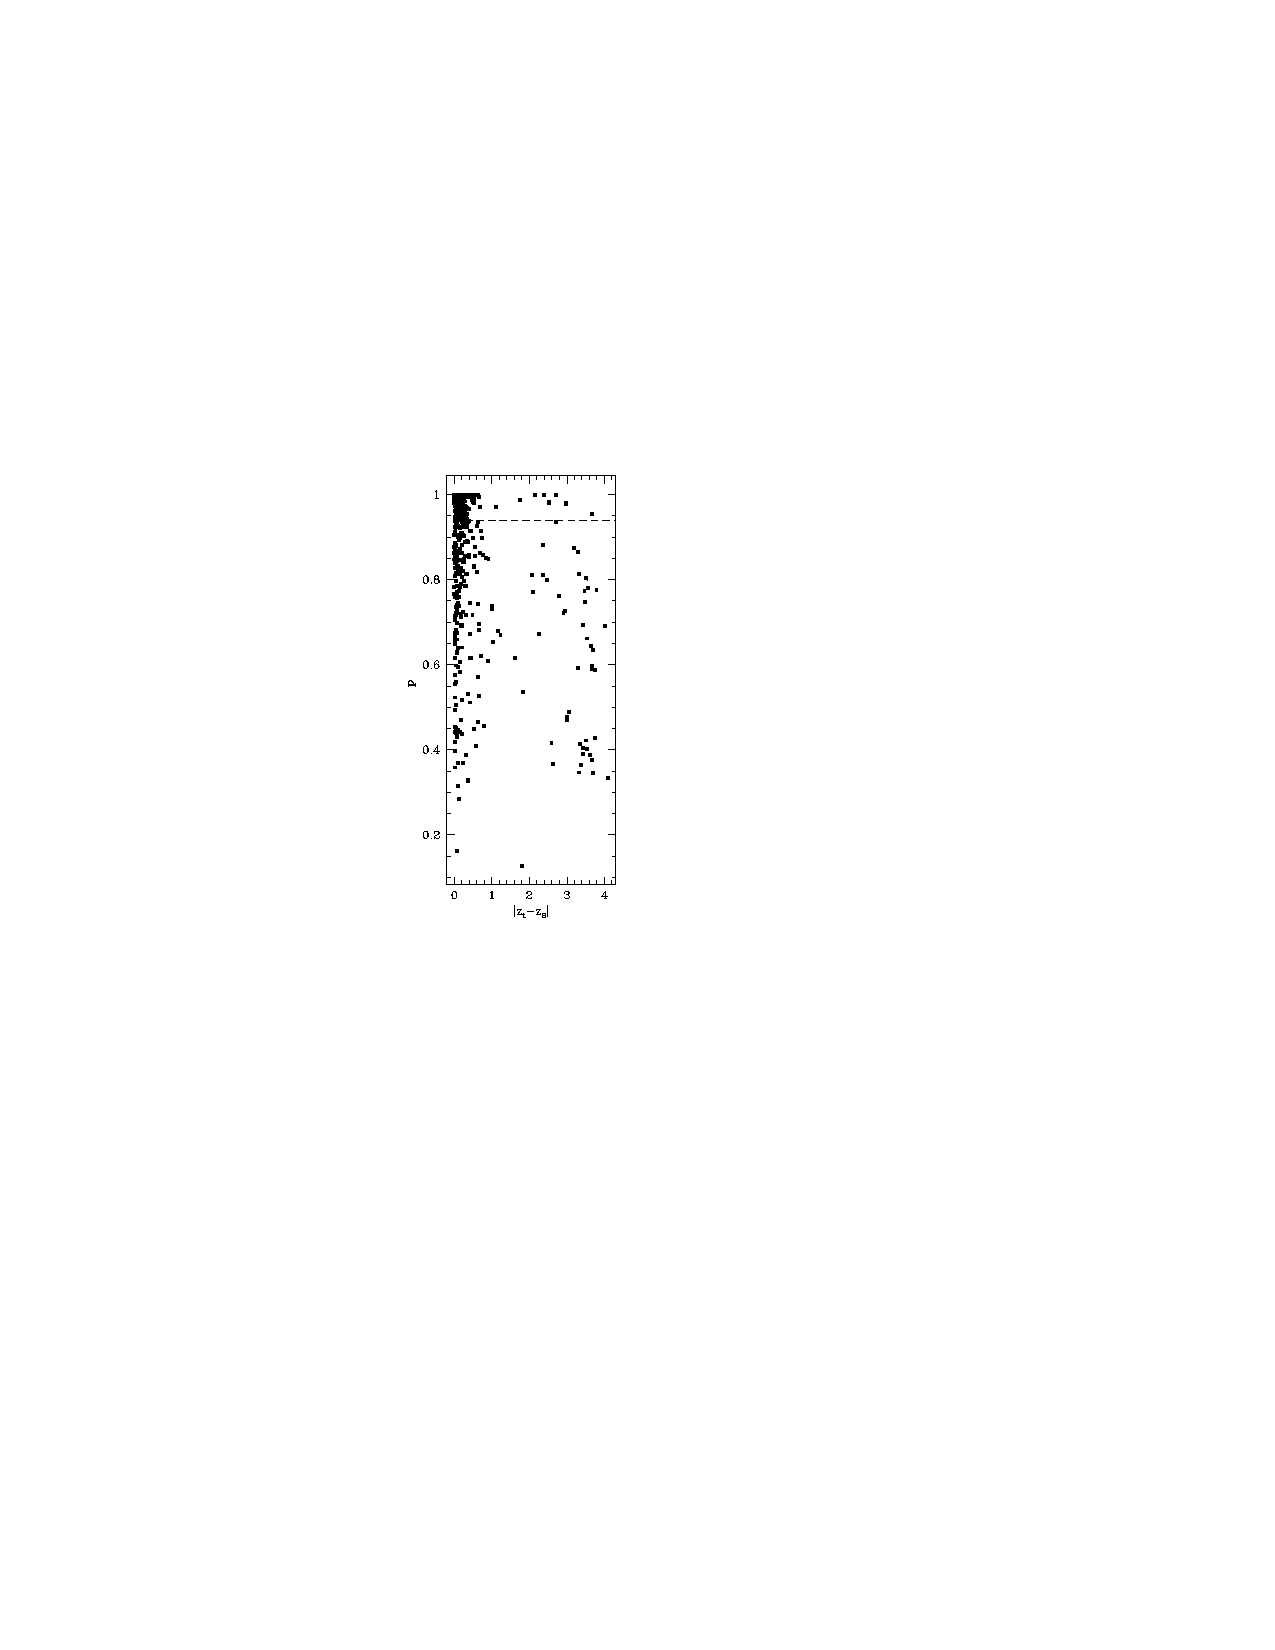
\includegraphics[height=76mm]{./plots/odds.pdf} & 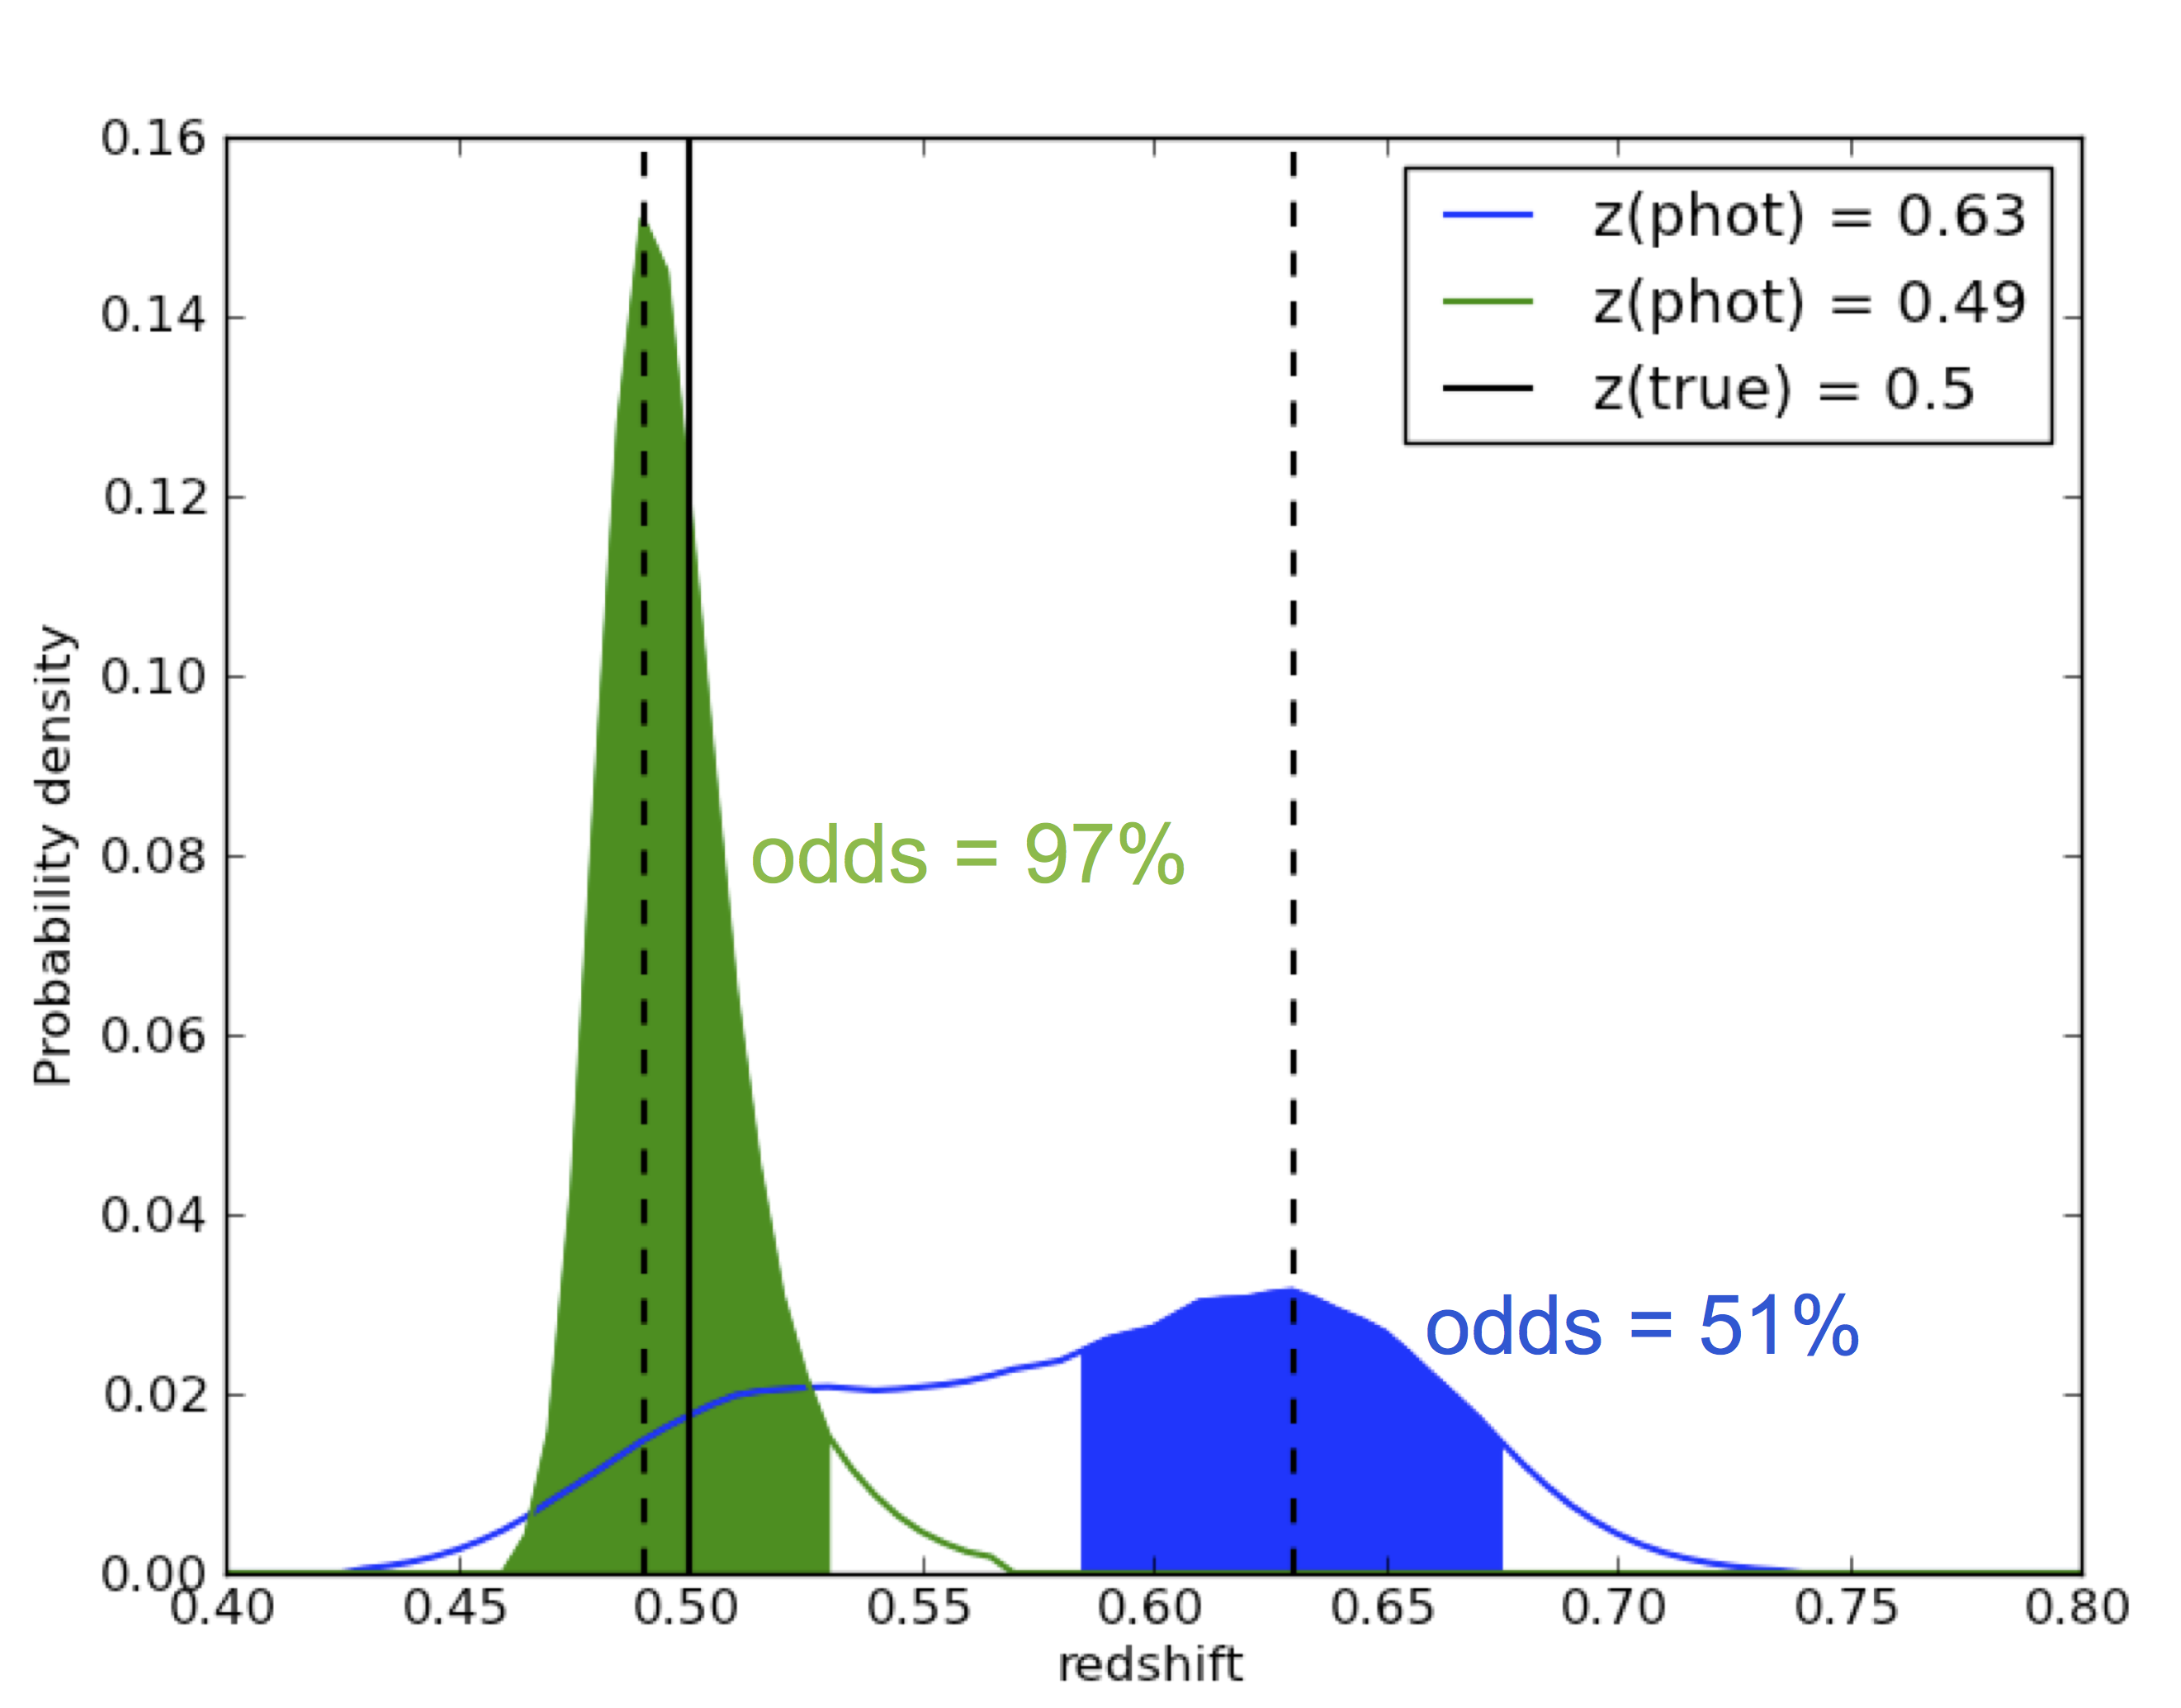
\includegraphics[height=80mm]{./plots/odds_example.png}
\end{tabular}
\caption{Left: Scatter plot of odds (shown as $p$) vs. $|z_{sp}-z_{ph}|$ for galaxies of the Hubble Deep Field (HDF). Points under the dashed line comprise 25\% of the catalog. Right: Two examples of $p(z|m_j)$ for two luminous red galaxies in the 2SLAQ sample whose spectroscopic redshift is roughly the same $z_{sp} = 0.5$ (solid black vertical line). Colored regions under the curves represent the area enclosed by the interval where the odds are computed. Dashed vertical lines show the best estimate of photo-$z$ given by BPZ (the mode of $p(z|m_j)$). Left plot from \citet{Benitez2000}.}
\label{fig:odds}
\end{figure}
